\documentclass[12pt]{article}
\usepackage[utf8]{inputenc}
\usepackage{graphicx} % Allows you to insert figures
\usepackage{amsmath} % Allows you to do equations
\usepackage{fancyhdr} % Formats the header
\usepackage[a4paper, total={6in, 8in}, margin=1in]{geometry}
\usepackage{algorithm}
\usepackage{algpseudocode}
\usepackage{hyperref}
\linespread{1.25} % about 1.5 spacing in Word
\setlength{\parindent}{0pt} % no paragraph indents
\setlength{\parskip}{1em} % paragraphs separated by one line
\usepackage[style=authoryear-ibid,backend=biber,maxbibnames=99,maxcitenames=2,uniquelist=false,isbn=false,url=true,eprint=false,doi=true,giveninits=true,uniquename=init]{biblatex} % Allows you to do citations - does Harvard style and compatible with Zotero
\urlstyle{same} % makes a nicer URL and DOI font
\AtEveryBibitem{
    \clearfield{urlyear}
    \clearfield{urlmonth}
} % removes access date
\AtEveryBibitem{\clearfield{month}} % removes months in bibliography
\AtEveryCitekey{\clearfield{month}} % removes months in citations
\renewbibmacro{in:}{} % Removes the "In" before journal names

\renewbibmacro*{editorstrg}{%from biblatex.def
  \printtext[editortype]{%
    \iffieldundef{editortype}
      {\ifboolexpr{
         test {\ifnumgreater{\value{editor}}{1}}
         or
         test {\ifandothers{editor}}
       }
         {\bibcpstring{editors}}
         {\bibcpstring{editor}}}
      {\ifbibxstring{\thefield{editortype}}
         {\ifboolexpr{
            test {\ifnumgreater{\value{editor}}{1}}
            or
            test {\ifandothers{editor}}
          }
            {\bibcpstring{\thefield{editortype}s}}%changed
            {\bibcpstring{\thefield{editortype}}}}%changed
         {\thefield{editortype}}}}}

\renewbibmacro*{byeditor+others}{%from biblatex.def
  \ifnameundef{editor}
    {}
    {\printnames[byeditor]{editor}%
     \addspace%added
     \mkbibparens{\usebibmacro{editorstrg}}%added
     \clearname{editor}%
     \newunit}%
  \usebibmacro{byeditorx}%
  \usebibmacro{bytranslator+others}}
  % The commands above from lines 20-49 change the way editors are displayed in books
\AtEveryBibitem{%
  \clearlist{language}%
} % removes language from bibliography
\citetrackerfalse
% Removes ibids (ibidems)
\DeclareNameAlias{sortname}{family-given} % Ensures the names of the authors after the first author are in the correct order in the bibliography
\renewcommand*{\revsdnamepunct}{} % Corrects punctuation for authors with just a first initial
\addbibresource{References.bib} % Tells LaTeX where the citations are coming from. This is imported from Zotero
\usepackage[format=plain,
            font=it]{caption} % Italicizes figure captions
\usepackage[english]{babel}
\usepackage{csquotes}
\usepackage{tocbasic}
\renewcommand*{\nameyeardelim}{\addcomma\space} % Adds comma in in-text citations
\renewcommand{\headrulewidth}{0pt}
\setlength{\headheight}{14.49998pt}

\newcommand\titleofdoc{String Matching Algorithms}
\newcommand\Author{Ramindu Walgama}

\begin{document}
\begin{titlepage}
   \begin{center}
        \vspace*{2cm} % Adjust spacings to ensure the title page is generally filled with text

        \Huge{\titleofdoc}

        \vspace{0.5cm}
        \LARGE{Assignment Report}

        \vspace{4 cm}
        \Large{\Author}

        \vspace{0.10cm}
        \normalsize{20201959 - 2020/CS/195}

        \vspace{0.10cm}
        \normalsize{2020cs195@stu.ucsc.cmb.ac.lk}

        \vspace{3 cm}
        \Large{Jul 19, 2022}

        \vspace{0.25 cm}
        \Large{Data Structures \& Algorithms III – SCS 2201}

       \vfill
    \end{center}
\end{titlepage}

\setcounter{page}{2}
\pagestyle{fancy}
\fancyhf{}
\lhead{\leftmark}
\rhead{\MakeUppercase{\titleofdoc}}
\rfoot{\thepage}

\tableofcontents

\newpage

\listoffigures
\listoftables

\newpage

\section{Introduction} % If you want numbered sections, remove the star after \section

String matching algorithms are used to find the occurrence of a given pattern in a given text. Below mentioned algorithms are considered algorithms for this assignment.
\begin{enumerate}
    \item The Naïve Algorithm(Brute Force Algorithm)
    \item The Knuth-Morris-Pratt Algorithm(KMP Algorithm)
    \item The Rabin-Karp Algorithm
    \item The Boyer-Moore Algorithm
    \item The Boyer-Moore-Horspool Algorithm
\end{enumerate}

Compared the above-listed algorithms in detail, the second chapter. Furthermore performance wise is analyzed in the third chapter, considering the theoretical as well as practical aspects. In the fourth chapter, the approach to the assignment is discussed briefly, including psuedo code, language selection, and small discription about the output format.

\newpage

\section{Comparison of Algorithms}
The Naïve Algorithm is a brute force algorithm that is not suitable for this task when considering the performance. The other four algorithms perform a pre-process before the execution of the process as shown in the below table \ref{algosummarytable}.
\begin{center}
    \begin{tabular}{ p{9cm} | p{2.5cm} | p{1.8cm} | p{1.7cm} }
        \hline
        \multicolumn{1}{p{9cm}}{\bfseries Algorithm} & \multicolumn{1}{p{2.5cm}}{\bfseries Founder \& the year} & \multicolumn{1}{p{1.8cm}}{\bfseries Pre-processing} & \multicolumn{1}{p{1.7cm}}{\bfseries Searching phase} \\ \hline \hline
        The Naïve Algorithm(Brute Force Algorithm) & - & - & O(m x n) \\ \hline
        The Knuth-Morris-Pratt Algorithm(KMP Algorithm) & Boyer \& Moore, 1977 & O(m) & O(m x n) \\ \hline
        The Rabin-Karp Algorithm & Rabin \& Karp, 1987 & O(m) & O(m x n) \\ \hline
        The Boyer-Moore Algorithm & Knuth et al., 1977 & O(m + \sigma) & O(m x n) \\ \hline
        The Boyer-Moore-Horspool Algorithm & Horpool, 1980 & O(m + \sigma) & O(m x n) \\ \hline \hline
    \end{tabular}
    \captionof{table}{The time complexity of String Matching Algorithms; \textcite{yi_chang_2015}}\label{algosummarytable}
\end{center}
\sigma = alphabet\ size\ of\ the\ pattern\ and\ text;\ m = size\ of\ the\ pattern;\ n = size\ of\ the\ text\\

KMP algorithm is more suitable when the pattern contains a fewer alphabet and the pattern contains substrings that are repeated in the pattern so that when part of the pattern matches with the text and the rest does not match, it won't start to search from the beginning and avoid another rematch \autocite{best_algo_quora}. Here, can't guarantee that the entered text and the pattern are similar to the above-mentioned points since the pattern is user input \autocite{kmp_rabin_karp}. The KMP algorithm is more reliable than the Rabin-Karp algorithm because there can be a collision during the hash table lookup and the hash function. The Boyer-Moore algorithm and the KMP algorithm are used widely \autocite{yi_chang_2015}. The Boyer-Moore algorithm is an efficient algorithm in both theoretical as well as practical aspects. The Boyer-Moore-Horspool Algorithm is a simplified algorithm of the Boyer-Moore algorithm. This performs well when the given alphabet is large and has proven that the Horspool algorithm achieves the best overall results in medical texts \autocite{lovis_baud_2000} which is much similar to the given dataset.

\newpage

\section{Performance}
In practical terms, algorithms, as mentioned earlier, have a big difference even though they have O(m x n) time complexity as mentioned in the above table where m is the length of the pattern and n is the length of the text which is clearly visible on the below-quoted table \ref{carve_fat11_data} and table \ref{carve_fat12_data} which has performed for different types of image datasets. Here the time measured in seconds.
\autocite{yi_chang_2015}.

\begin{figure}[h]
\centering
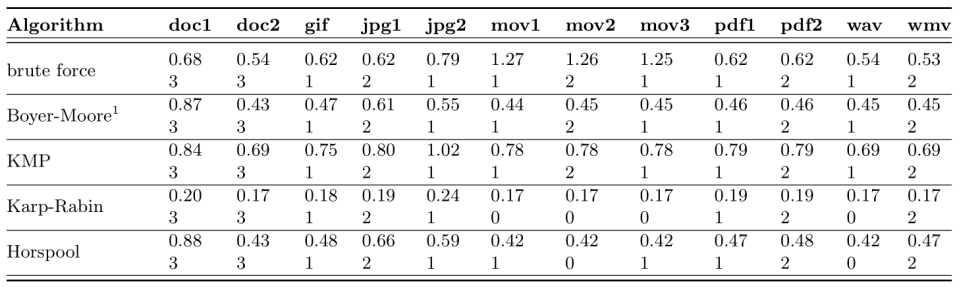
\includegraphics[width=\textwidth]{./images/Search Time (in secs) for Image “11-carve-fat.dd”.png}
\caption{Search Time (in secs) and Number of Files Carved for Image 11-carve-fat.dd \textcite{yi_chang_2015}}\label{carve_fat11_data}
\end{figure}

\begin{figure}[h]
\centering
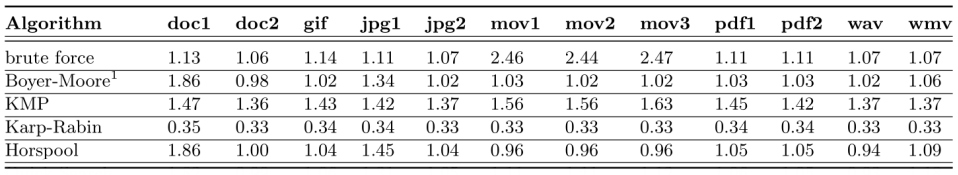
\includegraphics[width=\textwidth]{./images/Search Time (in secs) for Image “12-carve-fat.dd”.png}
\caption{Search Time (in secs) for Image “12-carve-fat.dd” \textcite{yi_chang_2015}}\label{carve_fat12_data}
\end{figure}

A better comparison can be done using comparison chart \ref{carve_fat11_chart} with respect to the table \ref{carve_fat12_data} above and chart \ref{carve_fat12_chart} with respect to the table \ref{carve_fat12_data} above. The data is drawn for other algorithms as well, which haven't been discussed in this report. According to the discussed algorithms, it is clear that the Boyer-Moore algorithm and the Boyer-Moore-Horspool algorithm perform better than the other discussed algorithms.

\begin{figure}[p]
\centering
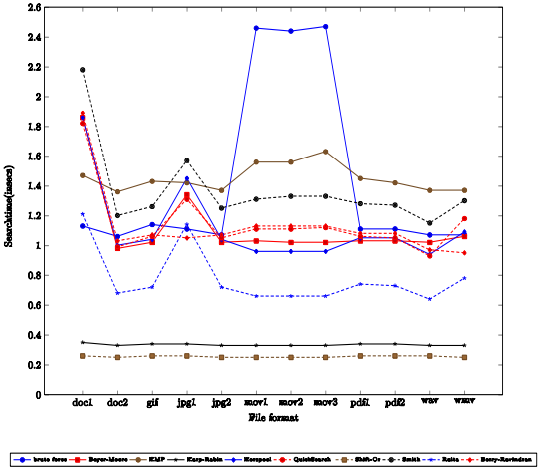
\includegraphics[width=\textwidth]{./images/Search Time Comparison for Image ”11-carve-fat.dd”.png}
\caption{Search Time Comparison for Image ”11-carve-fat.dd” \textcite{yi_chang_2015}}\label{carve_fat11_chart}
\end{figure}

\begin{figure}[p]
\centering
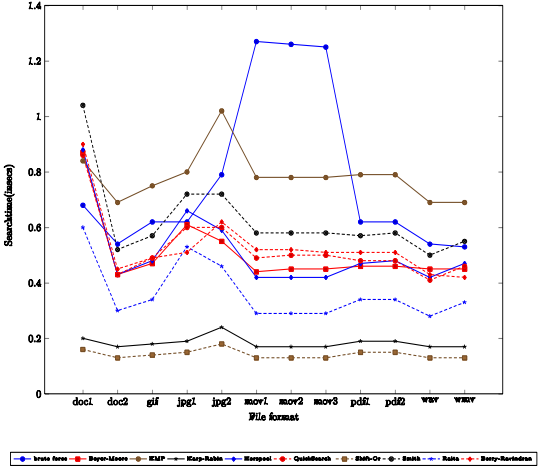
\includegraphics[width=\textwidth]{./images/Search Time Comparison for Image ”12-carve-fat.dd”.png}
\caption{Search Time Comparison for Image ”12-carve-fat.dd” \textcite{yi_chang_2015}}\label{carve_fat12_chart}
\end{figure}

\newpage

\section{Approach}
The Boyer-Moore-Horspool algorithm is used to complete this assignment by referring to the lecture slides, and other online material. The algorithm approach is very simple.

\subsection{Pseudo code}
Referred lecture notes and external sources such as \textit{\underline{ \href{https://www.cs.helsinki.fi/u/tpkarkka/teach/14-15/SPA/lecture05-2x4.pdf}{lectures of University of Helsinki}}}, \textit{\underline{\href{https://www-igm.univ-mlv.fr/~lecroq/string/node18.html}{lectures of Université Gustave Eiffel}}} and YouTube tutorials to understand and write the algorithm.
\begin{algorithm}
	\caption{The Boyer-Moore-Horspool algorithm}
	\begin{algorithmic}[1]
    	\Function{Horspool}{txt, pattern}
    	    \State $n \leftarrow$ length of the text
    	    \State $m \leftarrow$ length of the pattern
    		\For {$i=0,1,\ldots,\Sigma$}
    		    \State shift[$i]\leftarrow$m
    	    \EndFor
    	    \For {$i=0,1,\ldots,$m-1}
    		    \State shift[pattern[$i]]\leftarrow$m-$i-1$
    	    \EndFor

    	    \State $position_{txt} \leftarrow$ 0
    	    \While {$position_{txt} + m <= n$}
    	        \If {$txt[position_{txt} + m -1] = pattern[m-1]$}
    	            \State $position_{pattern} \leftarrow m -2$
                    \While {$position_{pattern} >= 0$ and $txt[position_{txt} + position_{pattern}] = pattern[position_{pattern}]$}
                        \State $position_{pattern} \leftarrow position_{pattern} - 1$
                    \If {$position_{txt} < 0$}
    	                \State pattern found
    	            \EndIf
                    \EndWhile
    	        \EndIf
    	        \State $position_{txt} \leftarrow position_{txt} + shift[txt[position_{txt} + m - 1]]$
    	    \EndWhile
    	\EndFunction
	\end{algorithmic}
\end{algorithm}

\newpage

\subsection{Language choose}
Used Python to implement the Boyer-Moore-Horspool algorithm. There are several reasons to choose the Python language. Python is widely used for data analytics, big data, and data science. Since here dealing with a large dataset, it is easy to visualise the output in many forms, such as different types of graphs and tables.

\subsection{Output}
The script required a single input from the user; a string to be searched in the "modules" dataset. After the execution, it will display the results in a table containing the line number of the matching string, module code, module name, number of matches in the same line, and the indices of the matches for that particular line. At the end, it will give a summary with the number of total occurrences and the number of total lines matched. The output for the input "Informatics" is shown below.

\begin{figure}[h]
\centering
\includegraphics[width=14cm]{./images/output-ss.png}
\caption{Script output for "Informatics" in modules.txt dataset}\label{output1}
\end{figure}

For to get the output as shown above a third party library, tabulate being used. Haven't any other libraries and this is used only for the ouput formatting.

\newpage

\section{Conclusion}
This report is mainly focused on the algorithms that are being taught within the 2201-DSA module but learned extra learnings by completing this assignment such as new algorithms which are not being discussed during the lectures and the comparisons of these algorithms to more extent.

\newpage

\printbibliography % If something looks strange in the bibliography, more often than not, you can modify the parameter in the .bib to fix the problem
\end{document}
